%%
%% This is file `sample-acmlarge.tex',
%% generated with the docstrip utility.
%%
%% The original source files were:
%%
%% samples.dtx  (with options: `acmlarge')
%% 
%% IMPORTANT NOTICE:
%% 
%% For the copyright see the source file.
%% 
%% Any modified versions of this file must be renamed
%% with new filenames distinct from sample-acmlarge.tex.
%% 
%% For distribution of the original source see the terms
%% for copying and modification in the file samples.dtx.
%% 
%% This generated file may be distributed as long as the
%% original source files, as listed above, are part of the
%% same distribution. (The sources need not necessarily be
%% in the same archive or directory.)
%%
%%
%% Commands for TeXCount
%TC:macro \cite [option:text,text]
%TC:macro \citep [option:text,text]
%TC:macro \citet [option:text,text]
%TC:envir table 0 1
%TC:envir table* 0 1
%TC:envir tabular [ignore] word
%TC:envir displaymath 0 word
%TC:envir math 0 word
%TC:envir comment 0 0
%%
%%
%% The first command in your LaTeX source must be the \documentclass command.
\documentclass[acmlarge]{acmart}
%%ss[STYLE]{acmart}
%% \BibTeX command to typeset BibTeX logo in the docs
\AtBeginDocument{%
  \providecommand\BibTeX{{%
    \normalfont B\kern-0.5em{\scshape i\kern-0.25em b}\kern-0.8em\TeX}}}

%% Rights management information.  This information is sent to you
%% when you complete the rights form.  These commands have SAMPLE
%% values in them; it is your responsibility as an author to replace
%% the commands and values with those provided to you when you
%% complete the rights form.
\setcopyright{acmcopyright}
\copyrightyear{2022}
\acmYear{2022}
\acmDOI{}


%%
%% These commands are for a JOURNAL article.
\acmJournal{POMACS}
\acmVolume{37}
\acmNumber{4}
\acmArticle{5}
\acmMonth{8}

%%
%% Submission ID.
%% Use this when submitting an article to a sponsored event. You'll
%% receive a unique submission ID from the organizers
%% of the event, and this ID should be used as the parameter to this command.
%%\acmSubmissionID{123-A56-BU3}

%%
%% The majority of ACM publications use numbered citations and
%% references.  The command \citestyle{authoryear} switches to the
%% "author year" style.
%%
%% If you are preparing content for an event
%% sponsored by ACM SIGGRAPH, you must use the "author year" style of
%% citations and references.
%% Uncommenting
%% the next command will enable that style.
%%\citestyle{acmauthoryear}

%%
%% end of the preamble, start of the body of the document source.
\begin{document}

%%
%% The "title" command has an optional parameter,
%% allowing the author to define a "short title" to be used in page headers.
\title{Paper Reading of \textit{Correlating Instrumentation Data to System States: A Building Block for Automated Diagnosis and Control}}

%%
%% The "author" command and its associated commands are used to define
%% the authors and their affiliations.
%% Of note is the shared affiliation of the first two authors, and the
%% "authornote" and "authornotemark" commands
%% used to denote shared contribution to the research.
\author{Yiwei Yang}
\email{yangyw@shanghaitech.edu.cn}
\orcid{0000-0001-8011-5868}
\affiliation{
  \institution{ShanghaiTech University}
  \streetaddress{1 R.D. Zhongke}
  \city{Shanghai}
  \state{Shanghai}
  \country{China}
  \postcode{21210}
}

%%
%% By default, the full list of authors will be used in the page
%% headers. Often, this list is too long, and will overlap
%% other information printed in the page headers. This command allows
%% the author to define a more concise list
%% of authors' names for this purpose.
\renewcommand{\shortauthors}{Yiwei Yang}

%%
%% The abstract is a short summary of the work to be presented in the
%% article.
\begin{abstract}
  The paper \cite{cohen2004correlating} talks about the use of Tree-Augmented Bayesian Networks (TANs) to identify system level metrics and thresholds which can define system states as high or low performant.

  The paper describes a method for developing an analytical engine that processes metrics and indicator values and, as a result, generates a classifier that predicts whether the system will meet SLOs or will fail to meet SLOs over time. Indirectly, the classifier determines the metrics that are most connected to SLO violations.
  As a result of this exercise, the metrics are modeled as a Bayesian network, with TANs used to reduce overfitting. To ensure that events are not modeled as mutually independent, the model is not chosen to be naive Bayes.

  Overall, TAN-based models have a high level of balanced accuracy, ranging from 87 to 94 percent. A single metric is insufficient to forecast patterns of SLO breaches (for example, in a model developed using naive Bayes). A limited set of (mutually dependent) measures, on the other hand, is sufficient to forecast SLO violations.
\end{abstract}

%%
%% The code below is generated by the tool at http://dl.acm.org/ccs.cfm.
%% Please copy and paste the code instead of the example below.
%%
\begin{CCSXML}
  <ccs2012>
  <concept>
  <concept_id>10010520.10010553.10010562</concept_id>
  <concept_desc>Distributed System~Peer to Peer System</concept_desc>
  <concept_significance>500</concept_significance>
  </concept>
  </ccs2012>
\end{CCSXML}

\ccsdesc[500]{}

%%
%% Keywords. The author(s) should pick words that accurately describe
%% the work being presented. Separate the keywords with commas.
\keywords{TAN, SLO}


%%
%% This command processes the author and affiliation and title
%% information and builds the first part of the formatted document.
\maketitle
\section{Strong point of the document}

\subsection{TAN use prior knowledge which increase the connection}
Models based on TANs are simpler to build than models based on prior knowledge. The paper's TAN models show a good connection between a small set of measures (3-8) and have a high accuracy of 90-95 percent.

TAN models are simple to copy and model, and they are versatile enough to accurately reflect real-world circumstances.

\begin{figure}[htbp]
  \centering
  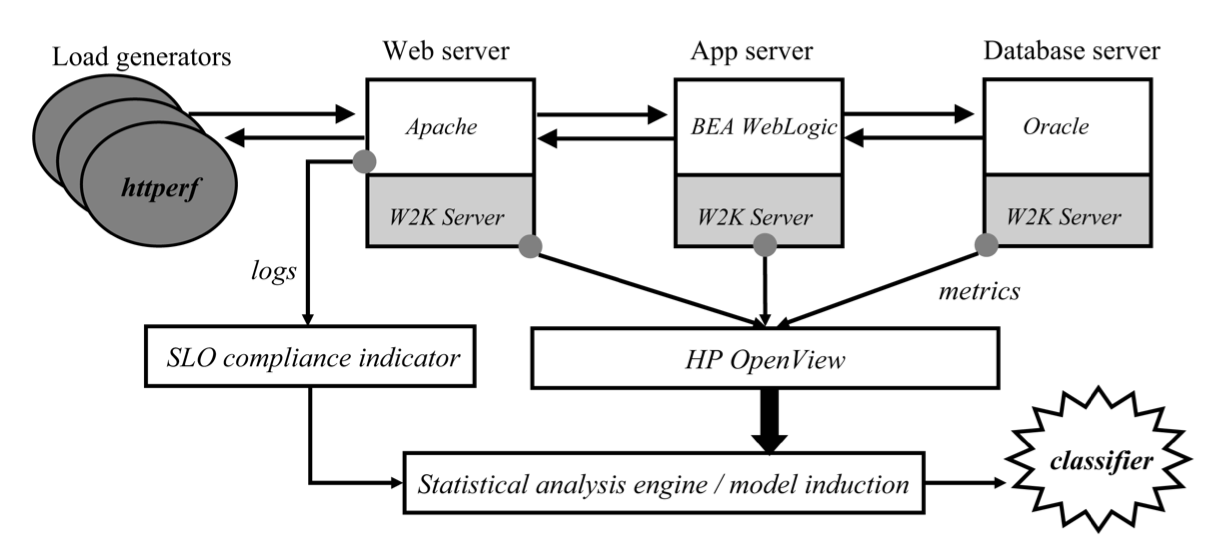
\includegraphics[width=0.3\columnwidth]{./overview.png}
  \caption{Overview of TAN based network \cite{cohen2004correlating}}
\end{figure}

\subsection{Implementation Detail}
Each node have a Tree Based Bayes Network to store the prior knowledge of metrics state. The classifier will classify the metrics into going to which state given which next packages.

$$\textbf{Metric}$$
$$\text{mean\_AS\_CPU\_1\_USERTIME}$$
$$\text{var\_AS\_CPU\_1\_USERTIME}$$
$$\text{mean\_AS\_DISK\_1\_PHYSREAD}$$
$$\text{mean\_AS\_DISK\_1\_BUSYTIME}$$
$$\text{var\_AS\_DISK\_1\_BUSYTIME}$$
$$\text{mean\_DB\_DISK\_1\_PHYSWRITEBYTE}$$
$$\text{var\_DB\_GBL\_SWAPSPACEUSED}$$
$$\text{var\_DB\_NETIF\_2\_INPACKET}$$
$$\text{mean\_DB\_GBL\_SWAPSPACEUSED}$$
$$\text{mean\_DB\_GBL\_RUNQUEUE}$$
$$\text{var\_DB\_NETIF\_2\_INBYTE}$$
$$\text{var\_DB\_DISK\_1\_PHYSREAD}$$
$$\text{var\_AS\_GBL\_MEMUTIL}$$
$$\text{numReqs}$$
$$\text{var\_DB\_DISK\_1\_PHYSWRITE}$$
$$\text{var\_DB\_NETIF\_2\_UTPACKET}$$

The balanced accuracy (BA) inherit, which averages the probability of correctly identifying compliance with the probability of detecting a violation.

$B A=\frac{P\left(s^{-}=\mathcal{F}(\vec{M}) \mid s^{-}\right)+P\left(s^{+}=\mathcal{F}(\vec{M}) \mid s^{+}\right)}{2}$

To choose a good bayesian classifier, the author used Markov Tree, in which they thought the CPU activity and IO activity is highly correlated to network traffic. Then to choose TAN model, they choose a linear time algorithm which provides latency assurance. With the correlation between network activity and TAN prediction, the author said it's highly interpretable and migratable.
\section{Weak point of the document}
\subsection{The metrics are human-chosen and requires cross validation}
Normally in a classification problem. we have to make the classification problem as well as possible, we have to verify those metrics have connection, so that we can remove some of them to maintain the runtime performance.
\subsection{The disk/network/CPU percentage is too generic to discover the underlying connections}
The connection between disk network CPU is too easy to say they have corralation. I would dig more metrics and system calls especially, to do the analysis.
\subsection{Other node is stateful which should be taken into account}The paper assumes most issues in a node to be caused by the node itself, and does not take into account the impact of different nodes in the system.
The paper assumes most issues in a node to be caused by the node itself, and does not take into account the impact of different nodes in the system.
\section{Possible Refinement to the idea}
\subsection{Deep Reinforcement Learning based network congestion prediction is more effective.}
\cite{jay2019deep} At each discrete time step $t \in 0,1, \ldots$, the agent observes a (locally perceptible) state of the environment $s_{t}$, and selects an action $a_{t}$. At the following time step $t+1$, the agent observes a reward $r_{t}$, representing its loss/gain after time $t$, as well as the next state $s_{t+1} \cdot^{2}$ The agent's goal is to choose a policy $\pi$ mapping states to actions that maximize the expected cumulative discounted return $R_{t}=\mathbb{E}\left[\sum_{t} \gamma^{t} \cdot r_{t}\right]$, for $\gamma \in[0,1)$. The parameter $\gamma$ is termed the discount factor. For large or continuous state and action spaces, this problem is intractable, and recent advances in deep RL employ deep neural networks to approximate the optimal $\pi$.
\subsection{Perfomance analysis today has way more tools to make thing better}
eBPF plus influx db could display the real time metrics on database, and those data could definitely be leverage.

\bibliographystyle{ACM-Reference-Format}
\bibliography{correlating_instrumentation_data_to_system_states_a_building_block_for_automated_diagnosis_and_control}
\end{document}